\documentclass[UTF8]{ctexart}
\usepackage{amsmath}
\usepackage{amsfonts}
\usepackage{amssymb}
\usepackage{graphicx}
\usepackage{hyperref}
\usepackage{float}
\usepackage{caption}
\usepackage{subfig}
\usepackage{bm}
\usepackage{mathrsfs}
\usepackage{latexsym}
\usepackage{euscript}
\usepackage{esint}

\renewcommand\thesection{\Roman{section}}

\hypersetup{colorlinks=true,linkcolor=black}

% Title Page
\title{距离平方反比定律的验证实验报告}
\author{17377306\ 马晓天}
\RequirePackage[a4paper]{geometry}
\geometry{
	textwidth=138mm,
	textheight=215mm,
	left=27mm,
	right=27mm,
	top=25.4mm, 
	bottom=25.4mm,
	headheight=2.17cm,
	headsep=4mm,
	footskip=12mm,
	heightrounded,
}


\begin{document}
\maketitle

\thispagestyle{empty}
\section{数据分析}
实验条件为：放射源(未记录)，探测器(型号未记录)，米尺(？分度)，高压电源为750V，放大器放大倍数为$1.0\times50=50 $，定标器阈值为0.49V。
实验原始数据为:
\begin{table}[H]
	\centering
	\caption{实验数据}
	\begin{tabular}{ccccccccccc}
		\hline
		$ R/m$ & 0.020 & 0.040 & 0.060 & 0.080 & 0.100 & 0.140 & 0.160 & 0.200 & 0.250 & 0.280\\
		\hline
		$ t_{\rm s}/\rm s$ & 10 & 20 & 20 & 30 & 40 & 60 & 70 & 80 & 90 & 100\\
		$ N_{\rm s}$ & 28186 & 32058 & 19459 & 20514 & 21139 & 23223 & 23554 & 23136 & 23127 & 26781\\
		$ n_{\rm s}/\rm s^{-1}$ & 2818.6 & 1602.9 & 972.95 & 683.80 & 528.48 & 387.05 & 336.48 & 289.20 & 256.97 & 267.81\\
		$ n_0/\rm s^{-1}$ & 2649.0 & 1433.3 & 803.35 & 514.20 & 358.88 & 217.45 & 166.88 & 119.60 & 87.37 & 98.21\\
		$ \sigma_{n_0}/\rm s^{-1} $ &16.8&9.0&7.10&4.95&3.86&2.85&2.55&2.30&2.13&2.09\\
		$ \log R$ & -1.70 & -1.40 & -1.22 & -1.10 & -1.00 & -0.85 & -0.80 & -0.70 & -0.60 & -0.55\\
		$ \log n_0$ & 3.423 & 3.156 & 2.905 & 2.711 & 2.555 & 2.337 & 2.222 & 2.078 & 1.941 & 1.992\\
		$ \sigma_{\log n_0} $ &0.003&0.003&0.004&0.0004&0.005&0.006&0.006&0.008&0.010&0.009\\
		\hline
	\end{tabular}
\end{table}
其中$ R $为探测器与放射源距离，$t_{\rm s}$为测量时间，$N_{\rm s}$为测量计数，$n_{\rm s}$为计数率，$ n_0=n_{\mathrm{s}}-n_{\rm b} $为净计数率，$ \sigma_{n_{0}} $和$ \sigma_{\log n_{0}} $为标准误差。环境本底测量时间$ t_{\rm b}=100\rm s $，计数$ N_{\rm b}=16960 $，计数率$ n_{\rm b}=169.60\rm s^{-1} $，标准误差$ \sigma_{n_{\rm b}}=1.30\rm s^{-1}$。
\subsection{绘制$ \log R-\log n_{0} $曲线}
为验证平方反比定律,假设:
\begin{equation}
n_{0}=\frac{C}{R^{m}}
\end{equation}
取对数得:
\begin{equation}
\log n_{0}=\log C-m \log R
\end{equation}
采用如下函数族进行拟合:
\begin{equation}
y=a x+b
\end{equation}
线性拟合得:
\begin{equation*}
a=-1.32\pm0.07,b=1.25\pm0.09,R^2=0.9788
\end{equation*}
比较式(2)(3)得:
\begin{equation}
m=-a=1.32\pm0.07
\end{equation}
拟合效果如图1，其中最右侧数据不合实际，拟合时舍弃。
\begin{figure}[H]
	\centering
	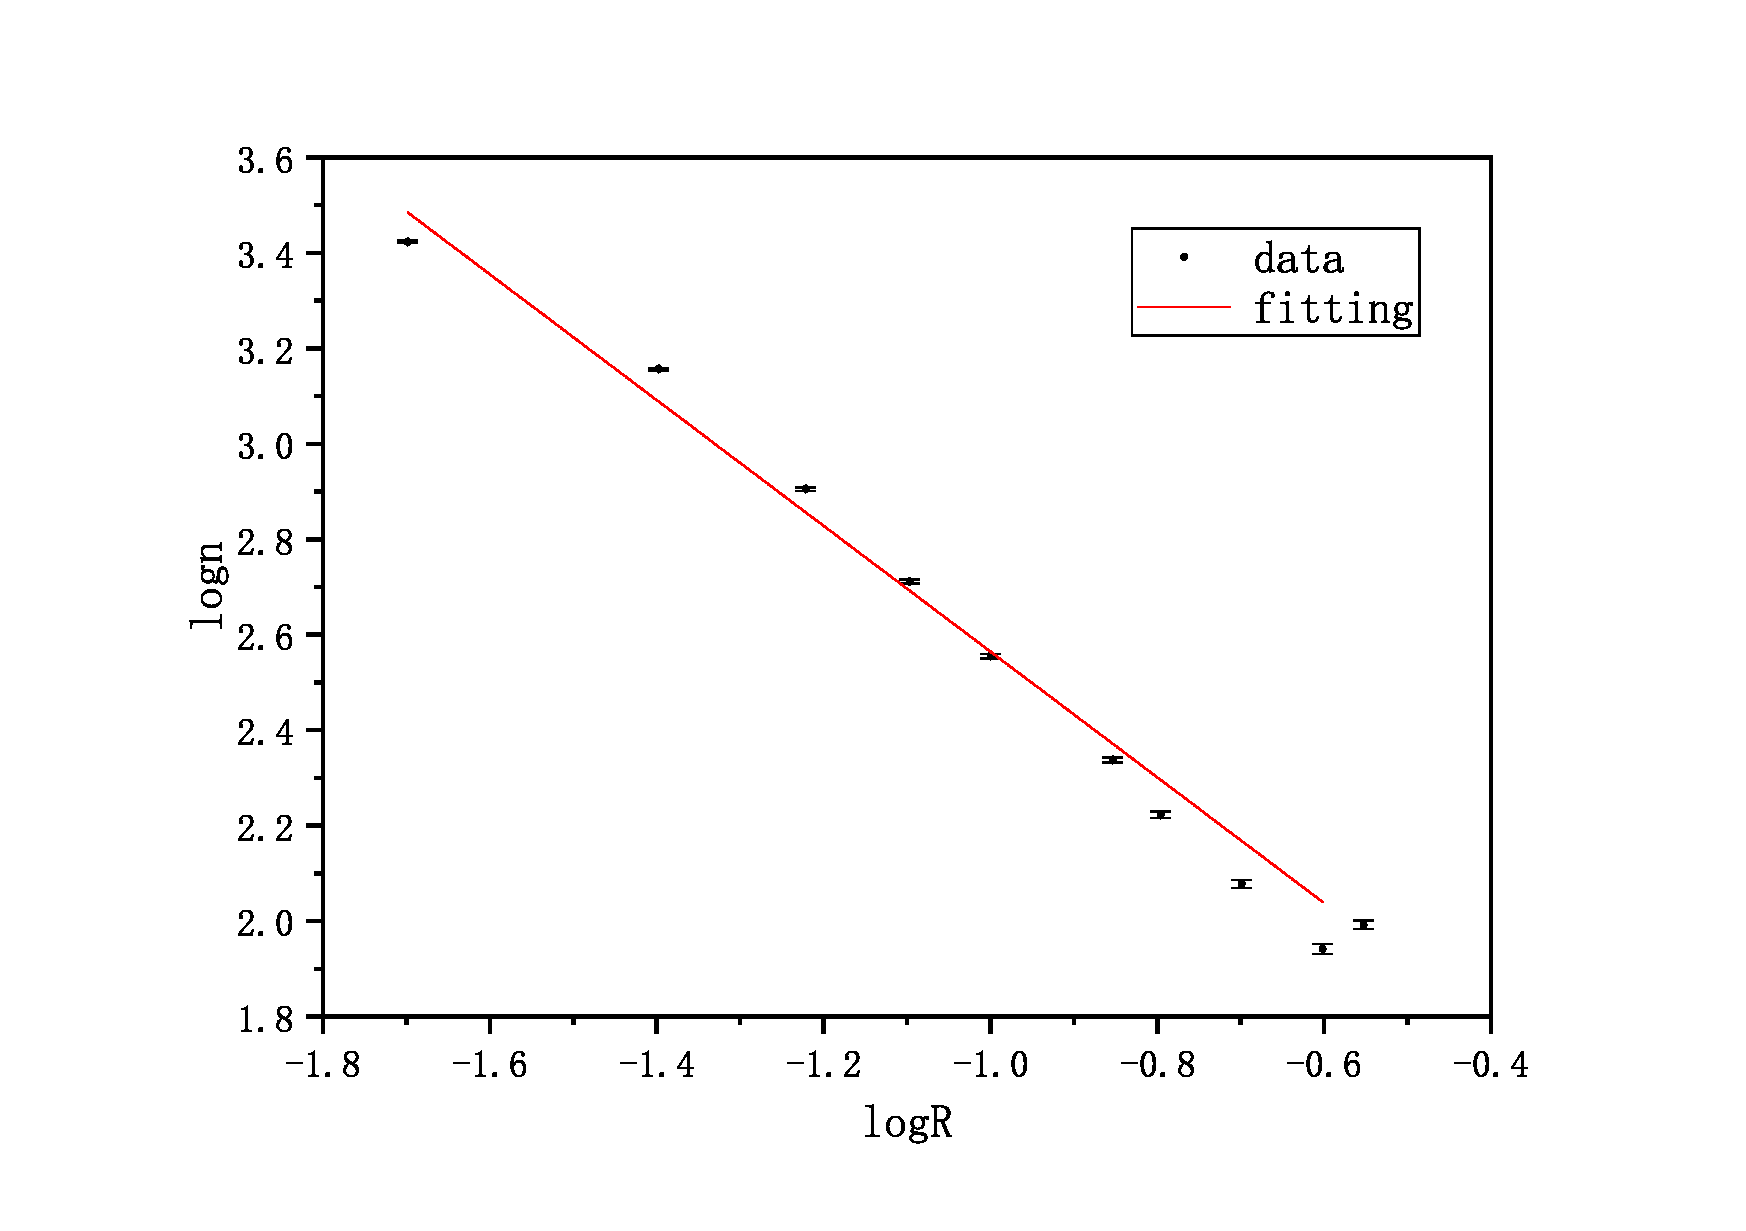
\includegraphics[width=0.9\linewidth]{logn0-logR.eps}
	\caption{$ \log n_{0}-\log R$曲线}
\end{figure}

\subsection{求出探测器探头与实际测量位置之间距离$ R_{0} $}
实际测量中，探测器探头与实际测量位置之间还应有$ R_0 $的距离需考虑，则实际需验证关系式为:
\begin{equation}
n_{0}=\frac{C'}{(R+R_0)^2}
\end{equation}
取对数得:
\begin{equation}
\ln n_{0}=\ln C'-2 \ln (R+R_0)
\end{equation}
为了求出$ R_0 $,采用如下函数族进行拟合:
\begin{equation}
y=a-2\ln(x+c)
\end{equation}
拟合得:
\begin{equation*}
a=1.811\pm0.041,c=0.027\pm0.001,R^2=0.9978
\end{equation*}
比较式(6)(7)得:
\begin{equation}
R_{0}=c=2.7\pm0.1(\rm cm)
\end{equation}
拟合效果如图2，最右侧数据拟合时舍弃。
\begin{figure}[H]
	\centering
	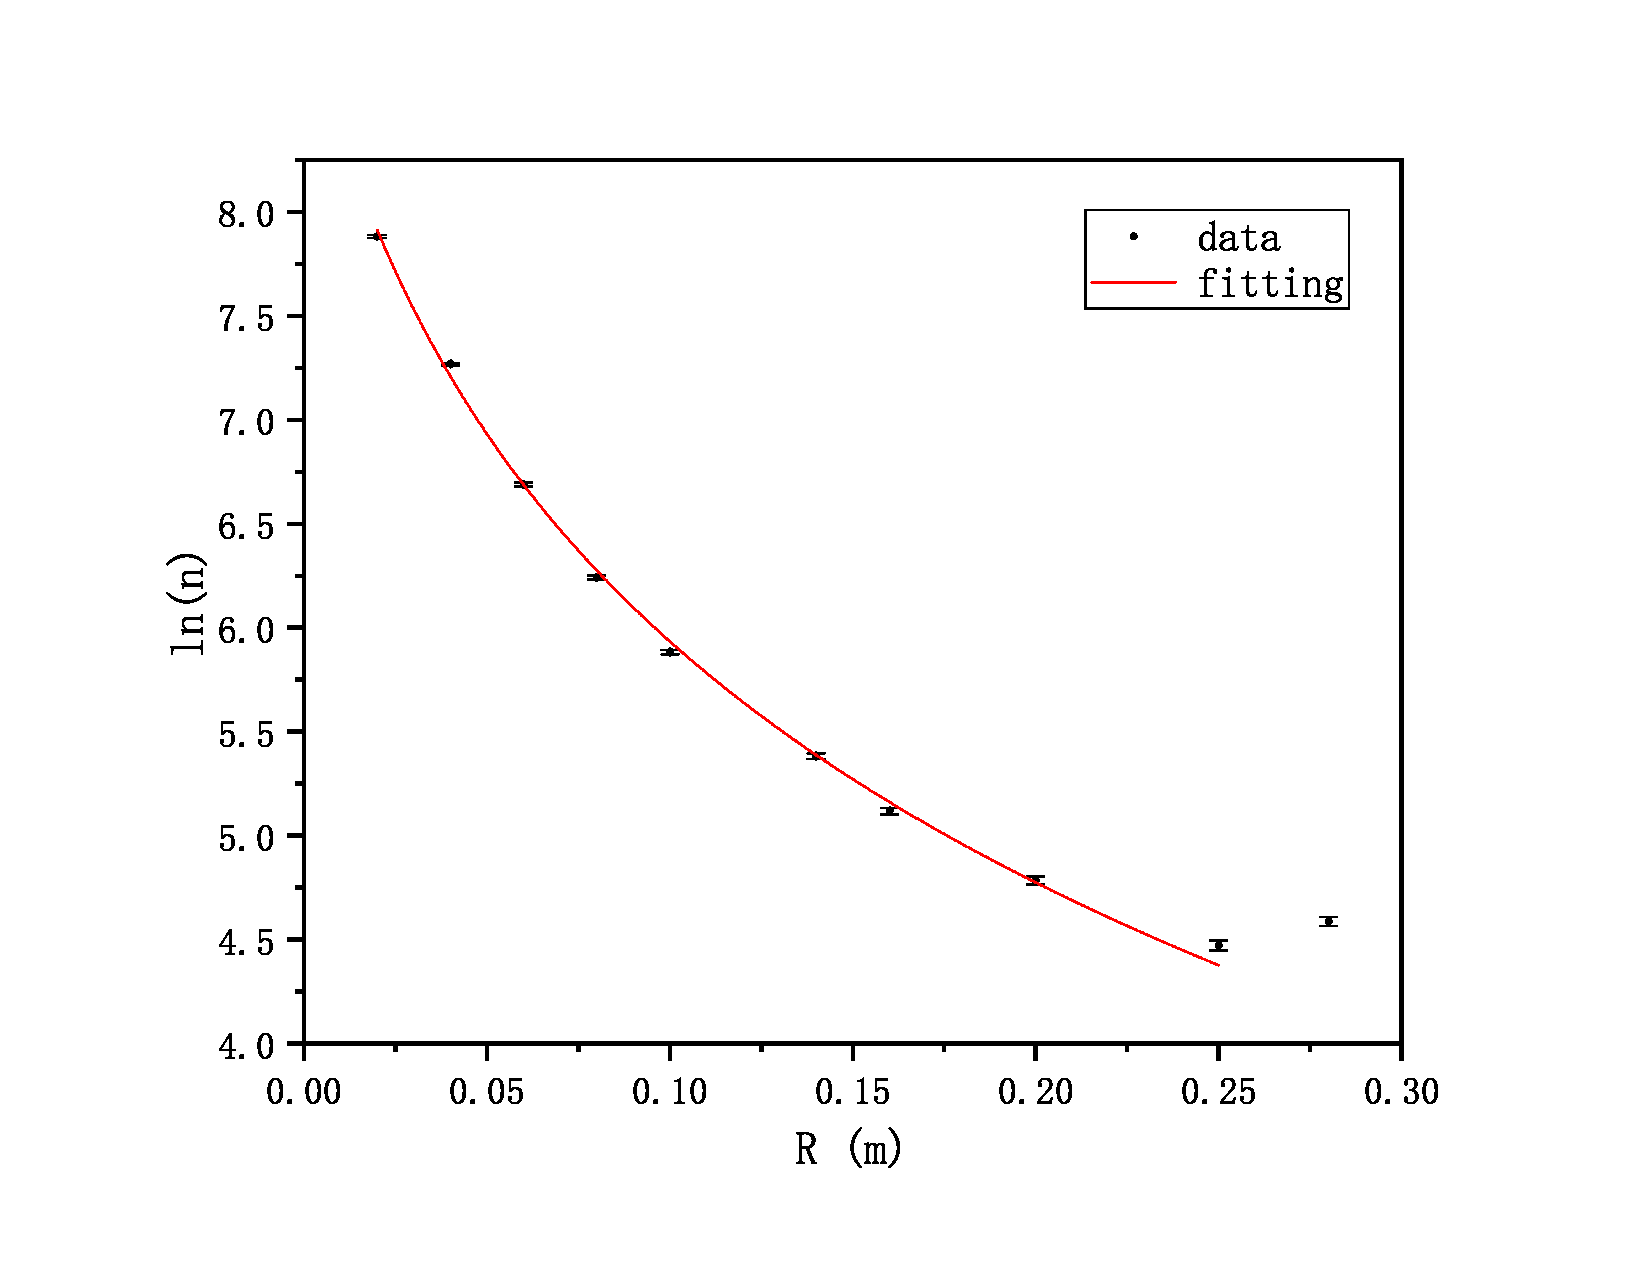
\includegraphics[width=0.9\linewidth]{R0.eps}
	\caption{$\ln n_{0}-R$曲线}
\end{figure}

\section{误差分析}
本次实验得到$ m=1.32\pm0.07<2$，经过分析得出误差的主要来源有：
\begin{itemize}
	\item[1.]
	探头有一定的面积
	\item[2.]
	探头与测量位置之间的距离$ R_{0} $\\
	上面已经分析并得到符合条件的$ R_{0}=2.7\pm0.1(\rm cm) $。
	\item[3.]
	距离的测量误差\\
	包括目测俯视仰视带来的读数误差，以及尺子与探测器的竖直线之间的夹角$ \theta $导致测量值与实际值有一定的差异。
	\item[4.]
	计数率的测量误差\\
	推测主要原因是调整触发电平时未调整好，示波器与电子计数器的计数频率差异较大。
\end{itemize}

\section{思考题}
\paragraph{1.本底计数率在改变位置后有没有变化，是否需要每次改变位置后重新进行测量？}
不变，因此无需在每次改变位置后重新测量。
\paragraph{2.对计数率进行多次测量，或者一次进行长时间测量，对计数率的精度有何不同？}
计数率的标准误差为$ \sigma_{\overline{n}}=\sqrt{\overline{n}/\sum_{i=1}^{N}t_{i}} $，则其相对标准误差为$\nu_{\overline{n}}=\sqrt{1/\sum_{i=1}^{N}N_{i}}$，由此公式可看出，如果一次测量和多次测量的总计数是一样的，那么精度就相同。总计数越少，精度就越低。

\section{实验总结}
本次实验探究了射线强度与距离的关系，了解了射线随距离以平方的速度衰减，掌握了放大、定标器、单道脉冲分析器等核心仪器插件的使用方法，加强了辐射防护中射线强度与距离关系的理解，收获颇多。同时，认识到理论与实际的差异，如在本实验中得到$ m \textless 2$，与理论有一定的差异，因为实际中探头那部分的距离未考虑进入。掌握了相关的数据处理和分析方法，并且在数据处理和撰写实验报告中熟悉了对Origin和\LaTeX{}的使用，实验和数据处理能力得到提升。

\end{document}